\chapter{An introduction to the writing of scientific texts} \label{chap:aChapter}
\begin{flushright}{\slshape    
   Science, my boy, is made up of mistakes, but they are mistakes
   which it is useful to make, because they lead little by little
   to the truth}. \\ \medskip --- \citeauthor{verne_journey:1957}
   \citetitle{verne_journey:1957} \citeyear{verne_journey:1957}
\end{flushright} 

\section{General rules}\label{sec:general_rules}
A scientific manuscript should be short, complete, clear, and logical.
It should convey the messages in the easiest, but still correct way.
Before writing, it may be useful to identify who the text is addressed to or the potential readers.
The type of readers should then lead the writing style. 
For example, the following type of text are all different, both for what concern the contents and the way the manuscript is organized:
\begin{description}
\item[a book] it is usually written for students;
\item[a scientific paper] it is written for peers: from scientists to scientists;
\item[a user manual] it is written for learning how to use a software, for example.
\end{description}

When writing the thesis, keep in mind that the reader is probably a person who knows about the specific research field, but does not know what you did, so do not take things for granted.

It may be useful to develop the text in different stages. 
First, define the structure of the text (see also Section \ref{sec:structure}).
Second, make a list of the main points in each section.
Then, further develop the list by sketching a couple of sentences for each point.
Finally, write the entire text.
This may be helpful to focus on the main contents of the text, the messages you would like to convey, and, not less importantly, to share and discuss the organization of the manuscript with your supervisor.

In general, each paragraph should convey one message. 
Try to keep the sentences short, because this will ease the reading and understanding process.
Avoid using phrases that are just a repetition, do not add any new message, or do not further contribute to understanding.
Avoid using synonyms: in scientific writing they may confuse the readers. 
For example: \\
\blockquote{We use a modeling framework composed of an optimization step followed by a simulation step. The modeling \sout{procedure} allows to analyze the system evolution.\\
We use a modeling framework composed of an optimization step followed by a simulation step. The modeling framework allows to analyze the system evolution.}

Use the active form if you are referring to what you did.
For example:
\blockquote{\sout{The HBV model is chosen because it is a parsimonious model.}\\
We chose the HBV model because it is a parsimonious model.}
The passive form, instead, is preferred to indicate what is done in the literature.
For example:
\blockquote{The HBV model is used because it is a parsimonious model.}

Be careful in using pronouns such as “it” or “they” to refer to a concept in the previous sentence. 
It is fine, if the previous sentence convey just one concept, otherwise the pronoun may be confusing.
In these cases, it is better to repeat the concept in the second sentence.
For example:
\blockquote{We assigned the same parameters to the different land use classes in the catchment. \sout{They} are taken from Wilson et al. (2014).\\
We assigned the same parameters to the different land use classes in the catchment. The land use classes are taken from Wilson et al. (2014).}

Bullet lists are welcome.
The items should be ranked following a rationale, for example they can be ranked by importance, preference, priority, etc.

\section{The structure of a scientific text}\label{sec:structure}
The typical structure is described in the following.
Nevertheless each thesis may have a different structure which can be customized to better highlight the work done.
Before writing the entire thesis, you should identify a temptative structure and discuss it with your supervisor (see Section \ref{sec:general_rules}).

\begin{description}
	\item[Introduction]
	The Introduction should introduce the reader to the argument developed in the thesis.
	It should set the context and the reason why the topic is interesting.
	State the research questions addressed in the thesis and the objectives of the work.
	The novelties of the work should also be highlighted.
	You can also briefly mention the methods used.

	\item[Literature review]
	It contains the description of previous works and what has been already done in the literature. 
	The text should be complemented with appropriate references (see Section \ref{sec:citations}). 

	\item[Materials and Methods]
	It should describe the methods and techniques employed to address the research questions, the workflows, the hypothesis, the experimental setting, etc.
	If you are using a specific dataset, you should introduce it in this section.
	In principle, any reader should be able to reproduce the work and experiments you did by reading this section.

	\item[Case study]
	If you are focusing on one or more case studies, this section should include the description of the study sites.
	Do not describe anything about the study site, but only include information that are relevant for your work, to understand what follows or why the application is relevant.

	\item[Results]
	This section should describe the results of the analysis.
	The text should be complemented with figures and tables, which are intended to support the evidences described in the text and to better comunicate the results (see Section \ref{sec:fig_and_tab}).

	\item[Discussion]
	This section contains the interpretations of the results and state the conclusions you can draw from the analysis.
	You should also discuss the limitations of your approach and identify future research paths.
	This section may be merged with the \enquote{Results} section.

	\item[Conclusion]
	You should make a short summary of the objectives of the work, the main results, and what you can conclude from your analysis.
	If you listed one or more research questions, you may want to formulate the reply which should be based, of course, on the evidences produced by your work.
	You can also briefly mention limitations and future works. 
\end{description}

\section{In-text citations}\label{sec:citations}
Citations usually goes just after the sentence you are quoting or paraphasing using brackets. 
The most commonly used type of citation is: author, year. 
When the reference has two or three authors of the source, cite all of them.
If there are more than three authors, you can cite the first author followed by \enquote{et al.} 
If the authors are subject of a sentence, only the year of publication is included in the brackets.
For example: \\
\blockquote{Air passing above a forested area is more humid than the one passing over a not forested area (Spracklen et al., 2012). \\
Spracklen et al. (2012) demonstrated an increase of moisture in the air that passes above a forested area than a not forested one. }

Do not copy and paste form other sources unless you are directly quoting from a work.
For example:\\
\blockquote{The approach is summarized by Philbrick and Kitanidis (1997): \enquote{Together modelling and optimization are sometimes called Systems Analysis.}}

\section{Acronyms}
Acronyms are welcome, but it is better not to over-use them. 
A text full of acronyms is difficult to read and may confuse the readers or force them to remember what they mean or to go back to the point where they are defined.
For example:\\
\blockquote{In the US, the notion of an NWO became popular after the terrorist attacks on the WTC. However, officials in NATO and the WTO rarely refer to an NWO in proceedings relating to the GATT, and it can be said that the MVTO, the MFN clause, and SROs have little to do with an NWO.\footnote{Example taken from \url{http://www.scribendi.com/advice/the_correct_use_of_acronyms.en.html}}}.

Acronyms should be always defined the first time they are used (this may not apply to very popular acronyms, \eg, NASA, IPCC, etc., which may remain undefined).
If you use the suggested \LaTeX\ environment, \verb!acronyms!, as explained in \mySubsec{subsec:special_env} you can avoid to remember which is the first time you used the acronym.
It does that for you.
For example:\\
\blockquote{In this thesis we adopt \acf{EMODPS}. \ac{EMODPS} is an approximate dynamic programming method that combines direct policy search and multi-objective evolutionary algorithms.} % I had to use acf because within the \blockquote, acronym is not able to recognize that is the first time i'm using the acronym... nevermind

Be consistent: once you defined an acronym, readers will expect that you use the acronym instead of the full description.
It is better to summarize all the acronyms in a dedicated table.
This is done automatically if you use write every acronym in the dedicated environment \verb!acronyms!.
You find the list after the table of contents.
The command transform the word into a link to the list for people for forget the meaning while reading.

\section{Figures and Tables}\label{sec:fig_and_tab}
Figures and tables can be used to present a large amount of information to the reader and can be used to assist communication.
Still, try to keep the minimum number of figures/tables.
Figures and tables are not self-explanatory. 
Use the text to focus on the important point the reader should draw from them.

Tables/figures should be sequentially numbered as they appear in the text (in other words, Figure 2 can not be cited before Figure 1).
They should appear close to the text where they are cited first.
All the figures/tables included in the thesis must be cited somewhere in the text.\footnote{\LaTeX\ is of great help here: for instance, you should not worry about number ordering. Specific code for figures as well as for tables is given in \mySubsec{subsec:special_env}.}

Each figure/table should be understood without reference to the text.
Captions should, then, contain a brief description of the figure's contents, for instance an explanation of the legend (see Figure \ref{fig:boxplot_quality}).

\begin{figure}[htbp]
\centering
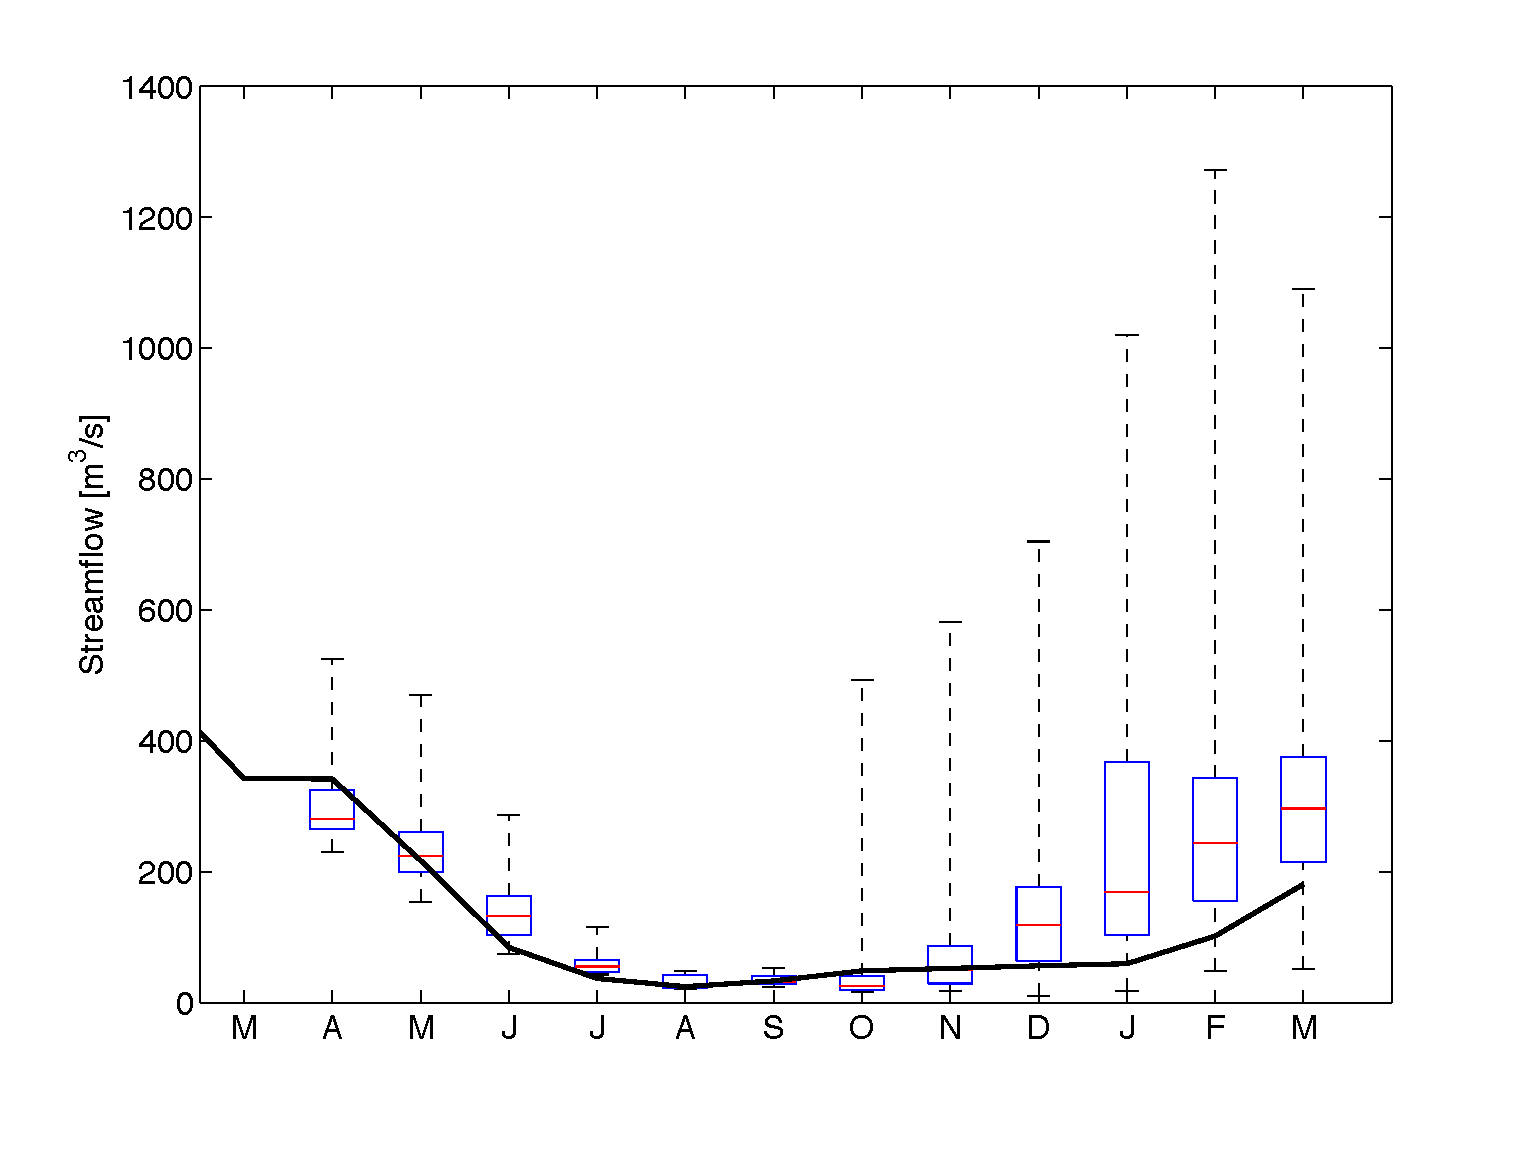
\includegraphics[width=\columnwidth]{Images/Introduction_Writing/boxplot_ensemble_2000.pdf} 
\caption[Streamflow forecast ensemble on April 1st 2000]{Streamflow forecast ensemble on April 1st 2000. The boxes show the 25\%, 50\%, and 75\% percentiles, while the whiskers represent the minimum and maximum ensemble members, thus indicating the full range of uncertainty. The solid black line represents the observations.}
\label{fig:boxplot_quality}
\end{figure}

Figures should always be good quality figures.
Axis tag, labels, and legend should have an appropriate font size.
Keep always the original figure (for example, \verb!.fig! if you created the figure with matlab): this will allow you or who is working with/after you to quickly modify it or recover the original data, if needed.
When applicable, keep the same axis ranges to the figures: it will ease the comparison between different figures.
When applicable/possible, use subfigures to ease the comparison between figures.

Finally, if you are using figures, tables and/or data from other sources, for example from other publications, cite always the reference. 
For example: \\
\blockquote{[...], taken/modified from Jones et al. (1950)}

\section{Mathematics}
Inline vs full line vs numbered equation.
Punctuation within equations.

Contemporary writers label the mathematical results in their papers as lemmas, theorems, propositions and so on.
Typically the major results of the paper are called theorems, the lesser results are called propositions.
The propositions are typically ingredients in the proofs of the theorems that are stand-alone statements of may be of independent interest), and the small technical results are called lemmas.
This probably varies quite a bit from writer to writer (and perhaps also from field to field).

\section{Margin notes}
Margin notes are used to study a new text or paper.
To read carefully a given text, it is essential that you write "all over" what you read, usually in the margins or between the lines?wherever there is space.
By annotating, you'll be creating a shorthand version of what you're reading to which you can return later for reference.
It's always much easier to navigate something you read a few days ago if you have taken detailed marginal notes.
We recommend to use margin notes when reviewing you own thesis.
Marginal notes help you to conceptualize the piece as you read.

Here are some general tips for annotating non-fiction articles.
Right next to each paragraph, write a brief phrase summarizing what happens in it. 
Underline passages that seem crucial to the point of the paragraph or to the larger thesis of the piece.
Note sections you don't fully understand with a question, like "What does this mean?" or "Doesn't this contradict my earlier argument?".
Outline points being made and the examples given to support them.
If you lists a number of reasons or factors that cause something or says something can be divided up into a certain number of parts, list the parts or factors in the margin.

\section{Submission to university: follow the instructions}
Visit \href{http://www.tedoc.polimi.it/tesilaurea/Consegna-tesi-di-laurea-(vecchio-ordinamento-e-specialistica)}{this link} for the updated information about the content of the thesis.

\enquote{Alcune Scuole forniscono linee guida specifiche cui i laureandi devono attenersi per la redazione della tesi. Per ulteriori informazioni:
\href{http://www.tedoc.polimi.it/download/lauree_magistrali/201406_POLITesi_Info_specifiche_scuole.pdf}{www.tedoc.polimi.it/\ldots}}

\subsection{Archiving electronic documents: PDF/A}
PDF/A is an ISO-standardized version of the Portable Document Format (PDF) specialized for the digital preservation of electronic documents. PDF/A differs from PDF by prohibiting features ill-suited to long-term archiving, such as font linking (as opposed to font embedding). The ISO requirements for PDF/A file viewers include color management guidelines, support for embedded fonts, and a user interface for reading embedded annotations.

Universities usually requires this standard but they're also not aware that common programs like MS Word, OpenOffice and so on aren't really able to produce compliant PDFs. In Latex, there's some development going on but at the time of writing, the available commands are still too obscure and buggy. So in the end, forget the PDF/A for now.\footnote{Or DIY and then make a pull request on github :D.}
